The \shell{makeinput}, \shell{compare}, and \shell{renderppm} subcommands are all functional.
More functionality may be added if necessary for efficient development, and potential changes have been outlined in the previous sections.

The \shell{fixedtime} headless simulation is functional, with each backend performing as intended. More optimization is intended (\cref{sec:Research:Optimization}), but the current program is fast enough to simulate the original ACA input at 120 ticks per second\footnote{On the researcher's GTX 1080. The program hasn't been tested on other systems.} which is a good baseline.

\begin{figure}[ht]
    \centering
    \centerline{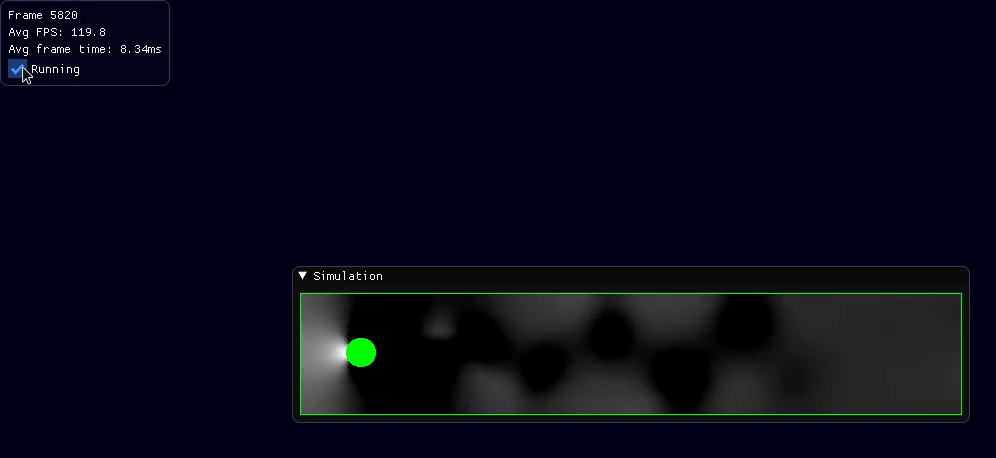
\includegraphics[width=1.25\linewidth]{Ch48Implementation/figures/example_running.png}}
    \caption{An example of the real-time visualization running on the ACA input}
    \label{fig:ExampleRunning}
\end{figure}
The visualized simulation creates a 1280x720 window and displays the simulation in a subwindow, which the user can move around.
The visualization is a simple display of the current pressure values, which is subpar (see \cref{sec:VizPressureCritique}), but this is planned to change.
A second window displays statistics about the last frame, and shows a checkbox which controls if the simulation is running as per \cref{req:VizPauseResume}.
As seen in this window, the simulation is running at 120 frames per second.
Each simulation tick is 1/60th of a second of simulation time, so the simulation is running at 2x real time.
This will be changed to account for \cref{req:VizSomeSpeed}.

